\documentclass[11pt]{article}
\usepackage[utf8]{inputenc}
\usepackage[T1]{fontenc}
\usepackage{amsmath}
\usepackage{amsfonts}
\usepackage{amssymb}
\usepackage[version=4]{mhchem}
\usepackage{stmaryrd}
\usepackage{graphicx}
\usepackage[export]{adjustbox}
\graphicspath{ {./images/} }

\begin{document}
\section*{Reading}
The Time Value of Money, Prices, and Rates

Cash is a financial asset that has an ultimate value that is based on its usefulness in obtaining real assets. Since the opportunities for converting cash into real assets change through time, cash flows to be received at different points in time are different commodities. This section, therefore, begins with a focus on the prices of prospective default-free cash flows.

\section*{Zero-Coupon Bond Prices and the Time Value of Money}
Consider a set of default-free zero-coupon bonds with $\$ 1$ face values (principal amounts) and with various maturities or longevities. In a perfect market with positive time value to money, a plot of the prices of these zero-coupon bonds against their longevities forms a monotonically declining function that asymptotically approaches zero as the longevities approach infinity. The next exhibit, Value of a Zero-Coupon Bond, depicts this relationship, which is often termed the present value function.

\begin{center}
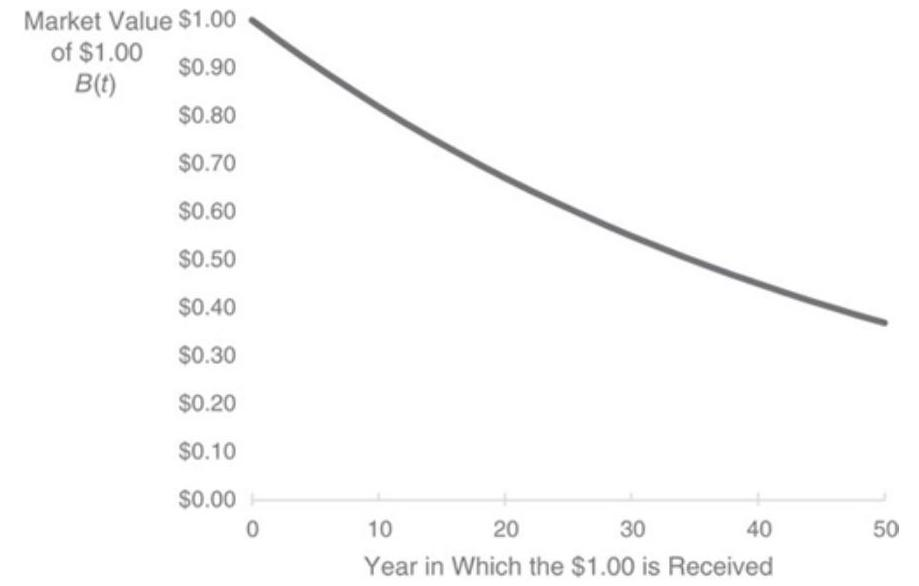
\includegraphics[max width=\textwidth]{2024_04_10_58b17af8323992df0cbag-2}
\end{center}

\section*{Value of a Zero-Coupon Bond}
The market price of $\$ 1$ due in $t$ years (i.e., a pure discount bond with a face value of $\$ 1$ ) is expressed as $B(t)$. Viewing the time value of money through the prices (as illustrated in the exhibit above), offers some advantages. However, the Value of a Zero-Coupon Bond exhibit does not effectively communicate the rates at which the prices change through prospective time. Therefore, most applications in finance express the time value of money through the lens of interest rates. Interest rates are used to enable improved intuition, yet they introduce substantial complexities due to issues such as compounding intervals. The Return and Rate Mathematics lesson discusses compounding assumptions in the context of return computation. The Deriving Interest Rates from Zero-Coupon Bond Prices section discusses compounding in the context of discount rates and, more generally, interest rates.

\section*{Deriving Interest Rates from Zero-Coupon Bond Prices}
Define $r_{t}^{m=1}$ as the interest rate corresponding to default-free cash flows due in $t$ years, calculated under the assumption of annual compounding (i.e., $m=1$ ). The rate can be calculated from the formula for a zero-coupon bond price based on annual compounding of interest:


\begin{equation*}
B(t)=F V\left(1+r_{t}^{m=1}\right)^{-t} \tag{1}
\end{equation*}


where $F V$ is the face value or principal amount of the bond.

For expositional simplicity assuming $F V=\$ 1$, then $r_{t}^{m=1}=B(t)^{-1 / t}-1$. More generally, for any finite compounding assumption with $r_{t}^{m}$ as the annual rate to be compounded $m$ times per year:


\begin{gather*}
B(t)=F V\left[1+\left(r_{t}^{m} / m\right)\right]^{-t m}  \tag{2}\\
r_{t}^{m}=\left\{[B(t) / F V]^{-1 /(m t)}-1\right\} m \tag{3}
\end{gather*}


Defining $r_{t}^{m=\infty}$ as the default-free interest rate corresponding to continuous compounding of the price, and continuing to assume the zero-coupon bond has a face value of $\$ 1$, the price and rate can be found as:


\begin{gather*}
B(t)=F V e^{-r_{t}^{m=\infty} t}  \tag{4}\\
r_{t}^{m=\infty}=-(1 / t) \ln [B(t) / F V] \tag{5}
\end{gather*}


Formulas 2 through 5 provide present values and interest rates for each compounding assumption. Continuous compounding is much easier to use once computational familiarity with the exponential function and the natural logarithmic function is achieved, although semiannual compounding is a convention in bond market quotations.

\section*{Determination of the Short-Term Interest Rate}
Although there is some evidence that markets price intraday lending, especially at times of crisis, the short-term interest rate generally refers to holding periods of one day, one week, or perhaps even one month. To the extent that a market is informationally efficient, the expected rate of return on various assets should be viewed on a real or after-inflation basis. The level of anticipated inflation is incorporated into any nominal rate of the time value of money. A nominal interest rate is the rate of return measured in terms of a given currency without a downward adjustment for the potential effects of positive inflation. Inflation is the rate of change in the value of a currency relative to a basket of real assets with a positive inflation rate indicating that the value of the currency is declining. The anticipated inflation rate $(\pi)$ is generally defined as a measure of the expected rate of change in the value of a currency measured through changes in overall price levels. Expectations of inflation rates vary across market participants and are generally unobservable. Accordingly, indications of anticipated inflation are often based on surveys of consensus estimates, derived from past inflation, or inferred from other market information such as interest rates.

The Fisher effect (or Fisher equation) states that the nominal interest rate $(i)$ is equal to the sum of the real interest rate $(r)$ and the expected inflation rate $(\pi)$, when interest rates are expressed as continuously compounded rates. The real interest rate is the annualized rate earned on default-free fixed-income investments, after adjusting the nominal rate downward for the effect of inflation. The real interest rate is usually expressed as an annualized short-term rate (e.g., daily or weekly) that is determined in the market by the supply and demand for short-term capital.

The traditional Fisher equation is sometimes modified for anticipated income taxes by assuming a uniform tax rate, $T$, on nominal interest income. The modified Fisher equation expresses the nominal interest rate (i) as the combination of the real interest rate, $r$, and the anticipated rate of inflation ( $\pi$ ), with an adjustment for the income tax rate, $T$, as shown in Equation 6:


\begin{equation*}
i=(r+\pi) /(1-T) \tag{6}
\end{equation*}


Equation 6 assumes that $r, i$ and $\pi$ are expressed as continuously compounded rates. If annualized rates are used a cross-term is introduced. Note that the Fisher equation is equal to the modified Fisher equation for the case of $T=0$.

The CAIA Level II curriculum discusses the determination of the term structure of interest rates, interest rate risk, and inflation risk in detail. This session turns to the issue of estimating the term structure of interest rates.

\section*{Estimating the Term Structure of Interest Rates with Zero-Coupon Bonds}
The term structure of interest rates is the relationship between spot interest rates and their associated longevities (i.e., times-to-maturity). The below exhibit depicts a common shape to the term structure of interest rates.

\begin{center}
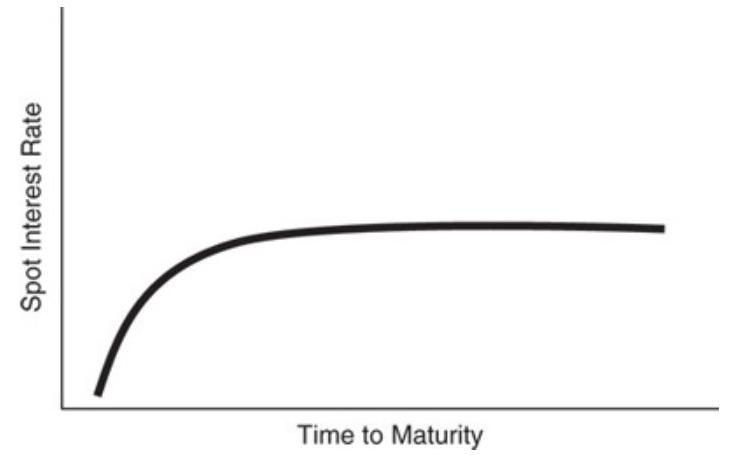
\includegraphics[max width=\textwidth]{2024_04_10_58b17af8323992df0cbag-3}
\end{center}

\section*{The Term Structure of Spot Interest Rates}
Given a large set of default-free zero-coupon bonds with a spectrum of maturities, the term structure can be estimated at each longevity corresponding to the maturities of the zero-coupon bonds. Fixed-income pricing focuses on yield to maturity. The yield to maturity of a fixed-income instrument is the rate that discounts all of the promised cash flows of the instrument into a summed present value that equals the instrument's market price.

In the case of a zero-coupon bond with face value $F V, T$ years to maturity, and a market price equal to $P_{T}$, the yield to maturity, $y$, can be determined with the following formula based on semiannual compounding:

$$
y=2\left[\left(\frac{P_{T}}{F V}\right)^{\frac{-1}{2 T}}-1\right]
$$

Note that, in the case of a zero-coupon bond, the preceding formula for yield is equivalent to the formula for the spot interest rate in the Deriving Interest Rates from Zero-Coupon Bond Prices section. Therefore, the yields of zero-coupon default-free bonds can be used to represent the term structure of spot interest rates.

\section*{The Yield Curve and Its Approximation}
Generally, fixed-income analysts wish to use coupon bonds to estimate most or all of the maturity ranges of the term structure of interest rates, because zero-coupon bonds are generally not available for longer maturities. A coupon bond with an annual coupon of $\mathrm{C}$ has the following formula for its price:


\begin{equation*}
P_{0}=\sum_{t=1}^{T} \frac{C}{(1+y)^{t}}+\frac{F V}{(1+y)^{T}} \tag{8}
\end{equation*}


The bond's yield to maturity (or simply its yield), $y$, is the rate that solves Equation 8 . Substituting $e^{y t}$ and $e^{y T}$ in place of the two denominators, respectively, generates an equation that can be solved for the yield expressed as a continuously compounded rate.

Note that a yield to maturity discounts each cash flow at the same rate regardless of its longevity and, therefore, is formed as a mixture of the spot rates associated with each cash flow. Yield to maturity does not have a market-based meaning except in the trivial case of a flat term structure of interest rates. In theory, each cash flow should be discounted with a rate associated with its longevity. However, yields are often used as a proxy for the term structure. In other words, yields-tomaturity are plotted against their corresponding terms-to-maturity and are described as yield curves that resemble the term structure of spot interest rates. Yields provide a somewhat close approximation to the spot rate corresponding to the bond's time-to-maturity, when coupon rates are small and when term structures are flat. However, for market environments with substantial coupons and sloped term structures, analysts often prefer to estimate spot rates. The next section discusses a method of deriving an estimate of the term structure of spot rates from coupon bonds.

Note however that in the case of zero-coupon bonds, the yield to maturity and the implied spot rate are identical because the zero-coupon bond has only one cash flow. Therefore, the zero-coupon bond's yield is not a mixture of rates from different times-to-maturity. Rather, it is a rate corresponding to a single time to maturity -the bond's time to maturity.

\section*{Bootstrapping the Term Structure of Interest Rates with Coupon Bonds}
Bootstrapping the term structure is the process of recursively estimating spot rates using one or more zero-coupon bonds on the short end and coupon bonds on the medium- and long-term regions of the term structure. The idea is to start with a short-term spot rate (i.e., a six-month zero-coupon yield) and use that rate to discount the first coupon of a one-year bond (with semiannual coupon payments). Since the one-year bond has only two cash flows (assuming semiannual coupons), the value of the second cash flow (the principal plus coupon payment in 12 months) can be found by subtracting the discounted value of the six-month cash flow from the total value (price) of the one-year bond.

For example, consider: (1) a six-month zero-coupon bond with a face value of $\$ 100$ and a price of $\$ 98$, and (2) a 12 -month $6 \%$ coupon bond with a face value of $\$ 100$, semiannual coupons and a market price of $\$ 102$. Note that the six-month zero-coupon bond is valued at $98 \%$ of its face value. The coupon bond's first coupon payment ( $\$ 3$ ) is due in six months and has a value of $\$ 2.94$, found by multiplying the $\$ 3$ coupon by $98 \%$ (the discount on six-month cash flows observed from the zerocoupon bond). The coupon bond also offers a $\$ 103$ cash flow in 12 months, with a value that must equal the excess of the coupon bond's total price (\$102) above the value of the coupon bond's first cash flow (\$2.94), which equals $\$ 99.06$. Note that the coupon bond's final cash flow is worth $96.175 \%$ of its undiscounted value (\$103). The final step is to convert the discount factor ( $96.175 \%$ or 0.96175$)$ into a one-year spot interest rate. The one-year spot rate can be expressed as $3.98 \%$ annually compounded, $3.94 \%$ compounded semiannually, or $3.90 \%$ compounded continuously.

The process could continue by analyzing an 18-month coupon bond, deriving the value of its final cash flow using the observed six-month and implied twelve-month spot rates, and converting the discounted value into an 18-month spot rate. Thus, an estimate of the entire term structure can be formed at six-month maturities if a bond can be found that matures on or very near each six-month interval.


\end{document}